\chapter{Metallurgie}	


\section{Metallurgie von Titan und Titanlegierungen (PH)}
Reines Titan ist das vierthäufigste Metall in der Erdkruste (etwa 0,4 -- 0,6 \%) und zeigt eine hohe Reaktivität mit anderen Elementen des Periodensystems. Es tritt in zwei verschiedenen Gittermodifikationen auf. Zum einen in der $\alpha$-Phase bei Raumtemperatur, die ein hexagonales Gitter annähernd dichtester Kugelpackung (hex) aufweist. Zum anderen in der $\beta$-Phase, die über einer Temperatur von $882 ^\circ C$ eine kubisch-raumzentrierte Gitterstruktur (krz) besitzt (Bild 1). Bei einer Temperatur von $882^\circ \pm 2 ^\circ C$ tritt eine Phasenumwandlung von $\alpha \arrowvert \beta$ auf. Die Temperatur, bei der diese Umwandlung stattfindet, ist eine wichtige Kenngröße im Bereich der Titanwerkstoffe und wird $\beta$-Transus-Temperatur ($T_{\beta}$) genannt.
Die Umwandlung $\beta \arrowvert \alpha$ kann durch einen diffusionskontrollierten Keimbildungs- und Wachstumsprozess erfolgen oder durch die Umwandlung durch einen diffusionslosen Umklappvorgang (martensitisch) erfolgen, wenn eine ausreichend schnelle Abkühlgeschwindigkeit (über 500 K/s) erziehlt wird (\ref{bib:}).

\begin{figure}[h]
	\centering
	\subfloat{}
	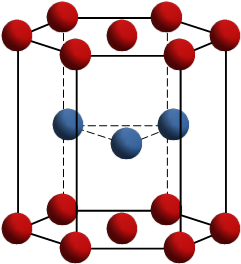
\includegraphics[width=0.3\textwidth]{Bilder/hcp}
	\hspace{4ex}
	\subfloat{}
	\includegraphics[width=0.3\textwidth]{Bilder/krz}
	\caption{Kristallgitterstruktur der $\alpha$-Phase (hex) und $\beta$-Phase}
	\label{fig:Kristallgitter}
\end{figure}


\subsection{Klassifizierung von Titan und Titanlegierungen}

Da reines Titan wie alle anderen Metalle keine hohe Festigkeit besitzt, werden Legierungen hergestellt, um die mechanischen Eigenschaften gezielt zu verändern. Die in der Industrie erhältlichen Titanlegierungen werden daher in verschiedene Klassen eingeteilt. Den $\alpha$-, $\alpha+\beta$- sowie den $\beta$-Legierungen. Die $\alpha+\beta$-Legierungen werden zusätzlich in near-$\alpha$- und near-$\beta$-Legierungen aufgeteilt. Die Klassifikation hängt vom Typ und der Menge der Legierungselemente ab. Des weiteren gibt es technisch reines Titan (CP-Titanium), das zunächst nur im amerikanischen Normungssystem ASTM (American Standard for Testing of Materials) in vier Klassen, den sogenannten CP-Grades 1,2,3 und 4 eingeteilt wurde. Dieses Bezeichnungssystem wurde später übersetzt und in deutsche und europäische Normen übernommen.
Die für Titanwerkstoffe typischen Legierungselemente werden in vier Kategorien eingeteilt, die sich in ihrer Wirkungsweise unterscheiden. 
Als alpha-Stabilisatoren werden Legierungselemente wie Aluminium (Al), Sauerstoff (O) und Stickstoff (N) bezeichnet, die zu einer Einschnürung des $\beta$-Phasengebietes führen und die $\beta$-Transus-Temperatur erhöhen.
Des weiteren gibt es die $\beta$-Stabilisatoren, die das $\beta$-Phasengebiet erweitern und die $\beta$-Transus-Temperatur verringern. Man unterscheidet bei den $\beta$-Stabilisatoren zwischen $\beta$-isomorphen und $\beta$-eutektoiden Stabilisatoren. Zu den $\beta$-isomorph wirkenden Stabilisatoren gehören die Elemte Molybdän (Mo), Vanadium (V), Niob (Nb) und Tantal (Ta). Diese erweitern das $\beta$-Phasengebiet bishin zur Raumtemperatur. 
Zu den $\beta$-eutektoiden-Stbilisatoren gehören Elemente wie Eisen (Fe), Chrom (Cr), Kupfer (Cu), Mangan (Mn) und Silizium (Si). Bei diesen Stabilisatoren kommt es unterhalb einer elementabhängigen Grenztemperatur zu einer eutektoiden Reaktion, die zu einer Ausscheidung einer zusätzlichen Phase führt. Diese Verbindung liegt entweder elementar oder intermetallisch vor.
Die Elemente  Zinn (Sn) und Zirkon (Zr) werden häufig als neutral bezeichnet, da diese nur eine sehr geringe $\alpha$-stabilisierende Wirkung haben.

\begin{figure}[h]
	\centering
	\includegraphics[width=1.0\linewidth]{"Bilder/Tabelle 1"}
	\caption[Tabelle 1]{Tabelle typischer Legierungselemte und ihre stabilisierende Wirkung [3,4]}
	\label{fig:tabelle-1}
\end{figure}


Bei einer Wärmebehandlung von near-$\alpha$-, $\alpha$+$\beta$- oder metastabilen $\beta$-Titanlegierungen im Zweiphasengebiet (also unterhalb der $\beta$-Transus Temperatur) kommt es bei ausreichend langen Glühzeiten zum sogenannten Element Partitioning [2]. Dabei diffundieren die $\alpha$-stabilisierenden Elemente in die $\alpha$-Phase und die $\beta$-stabilisierenden Elemente in die $\beta$-Phase, so dass die lokale chemische Zusammensetzung der jeweiligen Phasen, von der globalen chemischen Zusammensetzung einer Legierung, abweichen kann.

\begin{figure}[h]
	\centering
	\includegraphics[width=0.8\linewidth]{"Bilder/Tabelle 2"}
	\caption[Tabelle 2]{kommerziell genutzte Titanlegierungen nach ihren Erscheinungsjahren, der chemischen Zusammensetzung und maximalen Einsatztemperatur [9,10,11]}
	\label{fig:tabelle-2}
\end{figure}

\paragraph{$\alpha$ und near-$\alpha$-Legierungen}
Wenn $\alpha$-Stabilisatoren als Legierungselemente dem reinen Titan hinzulegiert werden, führt dies zu einer stabielen $\alpha$-Phase bei Raumtemperatur. Daher werden sie als $\alpha$-Legierungen bezeichnet. Wird ein kleiner Anteil an $\beta$-Stabilisatoren ( 1-2 Gew.\%) hinzugefügt, führt dies zu einer near-$\alpha$-Legierung mit einem kleinen Anteil an $\beta$-Phase bei Raumtemperatur. Ein typisches Beispiel einer $\alpha$-Legierung ist Ti–5Al–2.5Sn. Zu den Vertretern von near-$\alpha$-Legierungen gehören Ti–8Al–1Mo–1V und Ti–6Al–2Sn–4Zr–2Mo. Der Aluminiumgehalt in diesen Legierungen wird typischerweise unter 9 \% gehalten, da es sonst zu $Ti_{3}Al$-Ausscheidungen und dadurch zu Versprödungen kommen kann [1,2,3,4].

\paragraph{$\alpha$+$\beta$ Legierungen}
Diese Legierungen haben einen ausgeglichenen Anteil an $\alpha$- und $\beta$ Phase bei Raumtemperatur. Die bekanntesten $\alpha$+$\beta$ Legierungen sind Ti–6Al–4V und Ti–6Al–2Sn–4Zr–6Mo [1,2,3,4].

\paragraph{Near $\beta$- und $\beta$-Legierungen}
Diese Legierungen enthalten ca. 10--15 \% $\beta$-Stabilisatoren neben einem kleinen Anteil an $\alpha$-Stabilisatoren, haben dadurch einen größeren Anteil an $\beta$-phase bei Raumtemperatur und werden deshalb near-$\beta$-Legierungen genannt. Im Gegensatz dazu, haben die $\beta$-Legierungen einen sehr hohen Volumen-Anteil an $\beta$-Phase. Ein Beispiel für near-$\beta$-Legierungen ist Ti–5Al–2Sn–2Zr–4Cr–4Mo. Zu den Vertretern der $\beta$-Legierungen gehört Ti–15Mo–2.7Nb–3Al–0.2Si [3,4].

\paragraph{CP-Titanium} 
Zu reinem Titan werden keine Legierungselemente dazugegeben, jedoch sind Begleitelemente in bestimmten Mengen zugelassen und auch nicht zu vermeiden. In welche Klasse ein technisch reines Titan eingeordnet wird, hängt von der chemischen Zusammensetzung ab. Technisch reines Titan enthält neben Verunreinigungen nur Sauerstoff und Eisen als zusätzliche Legierungselemente.



\subsection{Herstellung von Titanlegierungen}
Titan kommt in der Natur nicht als reines Metall vor, sondern wird aus Titanerzen gewonnen. Die wirtschaftlich bedeutenden Erze sind Rutil ($TiO_2$) und Ilmenit ( $FeTiO_3$ - ein Gemisch aus Eisenoxiden und Titanoxiden), welche in allen Erdteilen zu finden sind. Einen Überblick über den Herstellungsprozess vom Erz bis zum Endprodukt ist in Abbildung 2 gegeben. Momentan ist das einzige Verfahren, um wirtschaftlich bedeutsame Mengen an Titan herstellen zu lassen, der Kroll-Prozess (bzw. der Hunter-Prozess) [1]. Beim Kroll-Prozess wird zunächst in einem Verhüttungsprozess das Titanerz von den Eisenoxiden getrennt. Dabei entsteht Roheisen, dass zur Produktion von hochwertigen Stählen genutzt wird, 
sowie Schlacke mit einem Titanoxidgehalt von etwa 80 - 90\%, die für die weitere Titangewinnung verwendet wird. Das in der Schlacke vorhandene Titanoxid wird unter der Verwendung von Chlorgas in mehreren Prozessschritten zu Titantetrachlorid ($TiCl_4$) umgesetzt. Dabei findet teilweise eine Rückreaktion zu $TiO_2$ statt, da Titan eine hohe Affinität zu Sauerstoff besitzt. Das Titantetrachlorid wird anschließend mit Magnesium (Einträufeln von flüssigem $TiCl_4$ in eine Magnesiumschmelze) zum sogenannten Titanschwamm (Sponge) reduziert. Dieser wird dann durch Vakuumdestillation von Rückständen (Mg und $MgCl_2$) befreit, aus dem Reaktionsgefäß gedrückt und zerkleinert. Der Titanschwamm wird dann unter Zusatz von Legierungselementen zu Elektroden verpresst, die in einem Vakuum-Lichtbogen-Umschmelzprozess (Vacuum-Arc-Remelting, kurz VAR), zu einem Block, dem Ingot, umgeschmolzen werden. Diese Ingots können dann weiterverarbeitet werden und zum Beispiel durch Techniken wie Schmieden oder Rollen zu Platten, Blechen und Streifen umgeformt werden. 

\begin{figure}[h]
	\centering
	\includegraphics[width=0.7\linewidth]{"Bilder/Abbildung 2"}
	\caption[Abbildung 2]{Überblick der Produktionsroute vom Erz zum Endprodukt [4]}
	\label{fig:abbildung-2}
\end{figure}

\pagebreak

\subsection{Mikrostrukturen in Titanlegierungen}
Im Bereich der Titanlegierungen gibt es vier Basis-Mikrostrukturen die geformt werden können. Es gibt Widmanstättengefüge, Bi-Modal/Duplex Gefüge, Globulare Gefüge sowie Martensitische Gefüge. Die $\beta$-Transus Temperatur spielt dabei eine entscheidene Rolle, welche Gefüge sich bei den Legierungen einstellen. Zusätzlich spielt die Abkühlrate beim Gießen der Legierung, der Grad beim heiß-/kaltumformen, die Glühtemperatur und Haltezeit eine wichtige Rolle [1,2,3,4]. 


Die Abbildung 6 {\ref} zeigt schematisch die Entstehung der Mikrostruktur von reinem Titan während des Gießprozesses. Es ist zu sehen, dass bei Abkühlung an der Luft unterhalb der Schmelztemperatur (1668$^\circ$C), sich $\beta$-phase in Form von Dendriten ausscheiden und zu kompletten $\beta$-Körnern wachsen. Bei weiterer Abkühlung bis unter $\beta$-Transus (882$^\circ$C für reines Titan), transformiert sich $\beta$ Phase zu $\alpha$, indem sich $\alpha$ Phase an den Korngrenzen absetzt und in Form von Lamellen ($\alpha$ Lamellen) in das vorherige $\beta$ Korn hineinwächst. Wenn mehrere dieser $\alpha$ Lamellen in dieselbe Richtung wachsen, formen Sie sogenannte $\alpha$ Kolonien. Diese Kolonien sind zufällig im vorherigen $\beta$ Korn verteilt und resultieren im sogenannten Widmannstätten Gefüge. Die Größe dieser mikrostrukturellen Formationen sind abhängig von der Abkühlrate. Schnelles Abkühlen unterhalb $\beta$-Transus resultiert in feinen $\alpha$ Lamellen und kleinen $\alpha$ Kolonien. Langsames Abkühlen führt zu breiteren Lamellen und gröberen Kolonien [1,2,3,4].

\begin{figure}[h]
	\centering
	\includegraphics[width=0.8\linewidth]{"Bilder/Abbildung 6"}
	\caption[Abbildung 6]{schematische Darstellung der Entstehung der Mikrostruktur in reinem Titan, abgekühlt aus dem flüssigem Zustand bis unter Beta-Transus [12]}
	\label{fig:abbildung-6}
\end{figure}


Mikrostrukturen, die man während des Gießens erhält, sind sehr grob und besitzen eine geringe Festigkeit. Daher werden diese Mikrostrukturen modifiziert mithilfe von Methoden wie thermo-mechanischer Verarbeitung, Wärmebehandlungen, die zu einer Verfeinerung der Mikrostruktur durch Rekristallisation führen oder durch Kornwachstum und Formation neuer Mikrostrukturen [1,2,3,4].
Typische thermo-mechanische Prozessschritte für Near $\alpha$ (Ti-6242) und $\alpha$+$\beta$ Legierungen (Ti-64) beinhalten die Homogenisierung (solution heat treatment), Deformation, Rekristallisation, das Altern (ageing) und Spannungsarmglühen (stress relief annealing) [1,2,3]. Ein Beispiel für den Ablauf dieser Prozessschritte ist in Abbildung 7 dargestellt. Diese Prozessschritte führen zu lamellaren, bimodalen und globularen Mikrostrukturen.

\begin{figure}[h]
	\centering
	\includegraphics[width=0.9\linewidth]{"Bilder/Abbildung 7"}
	\caption[Abbildung 7]{Prozessschritte für bimodale Mikrostrukturen von Alpha+Beta Legierungen schematisch [6]}
	\label{fig:abbildung-7}
\end{figure}

Eine kurze Beschreibung dieser Mikrostrukturen ist im folgenden aufgeführt.

- lamellare Mikrostruktur, entsteht bei einer Wärmebehandlung mit etwa 30 - 50 $^\circ$C über der $\beta$-Transus-Temperatur, nach plastischer Deformation im $\beta$ und $\alpha$+$\beta$ Phasengebiet, um große $\beta$körner zu vermeiden. Die resultierende Mikrostruktur ist abhängig von der Abkühlrate nach dem Glühen. So resultiert aus einer geringen Abkühlrate, eine grobe Widmannstätten Mikrostruktur, mit breiten $\alpha$-Lamellen, dickeren Korngrenzen und größeren $\alpha$-Kolonien.

\begin{figure}[h]
	\centering
	\includegraphics[width=0.7\linewidth]{"Bilder/Abbildung 3"}
	\caption[Abbildung 3]{lamellare Mikrostruktur von Ti-6242, Abkühlrate ca 100$^\circ$C/min, LM [2]}
	\label{fig:abbildung-3}
\end{figure}

\pagebreak

- bimodale Mikrostruktur, entsteht nach umfangreicher Deformation im $\alpha$+$\beta$ Phasengebiet und einer Wärmebehandlung unterhalb der $\beta$-Transus-Temperatur. Dies resultiert in globularem Primär $\alpha$ ($\alpha$-P), transformierten $\beta$ und $\alpha$ entlang der Korngrenzen der vorherigen $\beta$ Körner. Das transformierte $\beta$ besteht aus einer Widmannstätten Struktur, mit feinen $\alpha$-Lamellen, die in $\alpha$ Kolonien angeordnet sind. Die Größe dieser mikrostrukturellen Bestandteile hängen von der Glühtemperatur, Abkühlrate, sowie der Temperatur und Zeit bei der Deformation ab. Der Volumenanteil von primären $\alpha$ hängt haupsächtlich von der Temperatur beim Glühen und der Temperatur bei der Deformation ab [2].

\begin{figure}[h]
	\centering
	\includegraphics[width=0.7\linewidth]{"Bilder/Abbildung 4"}
	\caption[Abbildung 4]{bimodale Mikrostruktur Ti-6242, \SI{20}{\micro\metre}$}
	\label{fig:abbildung-4}
\end{figure}


- globulare Mikrostruktur, wird erreicht durch eine umfangreiche mechanische Bearbeitung im $\alpha$+$\beta$ Phasengebiet, sowie Lösungsglühen bei Temperaturen im Zweiphasengebiet, wo lamellares $\alpha$ in equiaxed $\alpha$ zerbricht, aufgrund des Rekristallisationsprozesses. Verlängertes Glühen vergröbert die equiaxed Mikrostruktur [2].

\begin{figure}[h]
	\centering
	\includegraphics[width=0.7\linewidth]{"Bilder/Abbildung 5"}
	\caption[Abbildung 5]{globulare Mikrostruktur von Ti-6242, LM [2]}
	\label{fig:abbildung-5}
\end{figure}



\subsection{Mechanische Eigenschaften von Titanlegierungen}

Dieser Abschnitt gibt einen Überblick über die typischen mechanischen Eigenschaften der verschiedenen Klassen von Titanlegierungen. Desweiteren werden die Einflüsse von verschiedenen Mikrostrukturen auf diese Eigenschaften aufgezeigt.

$\alpha$ Alloys - CP-Titanium ist das am weitesten genutzte unter den $\alpha$-Legierungen. Sie besitzen eine annehmbare Zugfestigkeit und gute Duktilität bei Raumtemperatur. Desweiteren besitzen sie eine geringere Dichte, eine gute Härte, sehr gute Kriechbeständigkeit und eine verbesserte Schweißbarkeit. Das Besondere an diesen Legierungen ist, dass sie bei kryogenen Temperaturen keine Veränderung von duktil zu spröde zeigen [1,2,4].

Near $\alpha$ Alloys - zeichnen sich durch eine hohe Kriech- und Oxidationsbeständigkeit aus. Ti-6242 ist die am häufigsten kommerziell eingesetzte Legierung für Temperaturen bis zu 450$^\circ$C.
Sie wurde als Ergänzung zu der bekannten Ti-64 Legierung entwickelt und erhöhte dadurch das Temperaturlimit. In den meisten Near $\alpha$ Alloys befindet sich Silikon (siehe Tab.2) als Legierungselement, um die Temperaturbeständigkeit zu verbessern [1,2].

$\alpha$ + $\beta$ Alloys - besitzen eine höhere Festigkeit, Härte und Korrosionsbeständigkeit. Dagegen ist die Duktilität und die Kriechbeständigkeit bei hohen Temperaturen nicht so gut, wie bei den near $\alpha$ Alloys. Diese Legierungen haben eine hohe Festigkeit bei Raum- und Mittleren Temperaturen, sowie gute Heißumformeigenschaften. Typischerweise besitzen diese Legierungen 10 - 15 \% an $\beta$ Phase bei Raumtemperatur. Bei über 20 \% werden sie schwer schweißbar. Ti-64 ist die meistverwendete $\alpha$ + $\beta$ Legierung und besitzt eine gute Kombination aus Festigkeit und Ermüdungseigenschaften bis zu 300$^\circ$C [3,4].

Near $\beta$ and $\beta$ Alloys - Near $\beta$ Alloys besitzen eine sehr gute Härtbarkeit und Formbarkeit über ein weites Band an Temperaturen. Sie haben eine hohe Festigkeit und Härte.
$\beta$ Alloy zeigen eine zusätzlich erhöhte Härte, Bruchzähugkeit und Korrosionsbeständigkeit.
Im Gegensatz zu den anderen Legierungen, haben sie eine hohe Dichte und eine geringere Duktilität. $\beta$ Alloys sind sehr anfällig für eine Duktil- zu Sprödumwandlung und daher nicht geeignet für den Einsatz bei niedrigen Temperaturen [1,2,4].

Die beschriebenen Eigenschaften der verschiedenen Legierungen sind jedoch abhängig von Faktoren wie den zugefügten Legierungselementen sowie dem gewählten Herstellungsprozess.
Durch zufügen einer beschränkten Menge von Legierungselementen, die sich in der Legierung auflösen/vermischen, kann es zu einer Erhöhung der Festigkeit durch Festlösungsverfestigung (solid solution strenghtening) führen. Werden Legierungselemente hinzugefügt, die nicht lösbar sind, formen diese zweite Phasen (intermetallic compounds), welche die Deformation einschränken und dadurch auch die Festigkeit erhöhen. Die Legierungselemente entscheiden größtenteils über die mechanischen und chemischen Eigenschaften (Korrosion, Oxidation) [1,2,4].

Der Herstellungsprozess hat ebenfalls einen erheblichen Einfluss auf die mechanischen Eigenschaften der Legierungen. Durch verschiedene Wärmebehandlungen können dadurch verschiedene Mikrostrukturen eingestellt und ihre mikrostrukturellen Eigenschaften verändert werden [1,2,3,4].

Wie im vorherigen Kapitel erwähnt, werden die Mikrostrukturen eingeteilt in lamellar, equiaxed und bi-modal. Diese bestehen hauptsächlich aus $\alpha$- und $\beta$phase, welche in verschiedenen physischen Formen auftreten. Die wichtigsten Eigenschaften der Mikrostrukturen werden durch die Faktoren Primär $\alpha$, $\alpha$ Kolonien, der Korngrenzen sowie dem transformierten $\beta$ beeinflusst [1,2,3]. Der Effekt der Mikrostrukturen auf die mechanischen Eigenschaften, abhängig von der mikrostrukterellen Größe der Faktoren, ist in Tabelle 3. aufgeführt. Die Größe der $\alpha$ Kolonien, welche aufgrund verschiedener Abkühlraten entstehen, ist der wichtigste mikrostrukturelle Faktor. Es hat sich gezeigt, dass eine Verringerung der Koloniegröße, zu einer Verringerung der effektiven Gleitebene führt. Dadurch wird die Streckgrenze erhöht und die Rissanfälligkeit verringert. Größere $\alpha$ Kolonien erhöhen dagegen den Widerstand gegen Ermüdungsrissausbreitung und die Bruchzähigkeit. Der Grund dafür liegt in den gröberen $\alpha$ Kolonien, die eine bessere Möglichkeit haben, den Riss abzulenken und daraus eine geringere Rissbildungsrate resultiert [1,2,4]. Die Größe der $\alpha$ Kolonien wird durch die Größe des vorherigen $\beta$-Korns limitiert. Daher führen größere vorherige $\beta$körner auch zu einer besseren Kriechbeständigkeit.

\begin{figure}[h]
	\centering
	\includegraphics[width=0.9\linewidth]{"Bilder/Tabelle 3"}
	\caption[Tabelle]{Effekt der Mikrostrukturen auf die mechanischen Eigeschaften in Abhängigkeit der Größe [3]}
	\label{fig:tabelle-3}
\end{figure}

\pagebreak

\subsection{Verwendung von Titan und Titanlegierungen}
Titanlegierungen werden hauptsächlich in der Luftfahrt- und Raumfahrt verwendet, da sie eine gute Kombination aus einem niedrigem Gewicht, hoher Festigkeit, Korrosionsbeständigkeit und einer hohen Temperaturstabilität bieten [1,5,6]. Die Haupteinsatzgebiete in der Luftfahrt für Titanlegierungen sind Strukturteile der Luftfahrzeugzelle, Fahrwerksteile sowie Komponenten von Flugtriebwerken. Etwa 7 - 36 \% des strukturellen Gewichts des Rumpfes und der Triebwerke bestehen aus Titanlegierungen [2]. In Triebwerken werden Titanlegierungen für Triebwerksschaufeln eingesetzt. Für die meisten Komponenten wird die Standardlegierung Ti-6Al-4V verwendet. Für Komponenten, die eine höhere Temperaturbeständigkeit erfordern, werden Legierungen wie Ti–6Al–2Sn–4Zr–2Mo und IMI 834 verwendet. Die hohen Material- und Herstellungskosten verhindern einen breiten Einsatz von Titanwerkstoffen in der Automobilindustrie. Sie werden aber vereinzelt für Motorkomponenten oder Fahrwerksteile, wie beispielsweise Federn benutzt. Technisch reines Titan (CP-Titanium) findet Anwendung in Bereichen, wo die Anforderungen an mechanische Eigenschaften gering, aber eine hohe Korrosionsbeständigkeit gefordert ist. Beispiel dafür sind Wärmetauscher, Rohrleitungen oder Meerwasserentsalzungsanlagen [7]. Desweiteren finden CP-Titanium und Titanlegierungen Anwendung in der Medizintechnik, aufgrund der Biokompalibität von Titan, sowie einer guten Dauerfestigkeit und Korrosionsbeständigkeit. Sie werden zur Herstellung von Implantaten sowie medizinischen Geräten benutzt [8]. Ein weiteres Einsatzgebiet sind moderne Schutzwesten, die neben den Aramidfasern auch Titangewebe enthalten, um das Eindringen von Hieb- und Stichwaffen zu verhindern [1]. 


[1] C. Leyens, M. Peters, Titanium and titanium alloys: fundamentals and applications, VCH Verlagsgesellschaft Mbh, 2003. [2] G. Lutjering, J.C. Williams, Titanium, Springer Verlag, 2007. [3] R. Boyer, G. Welsch, E. Collings, Materials Property Handbook: Titanium Alloys, ASM international, Ohio, USA, 1994. [4] M.J. Donachie, Titanium: A Technical Guide, Second ed., ASM International, Ohio, USA, 2010. [5] R.R. Boyer, An overview on the use of titanium in the aerospace industry, Materials Science and Engineering A 213 (1996) 103–114. [6] M. Peters, J. Kumpfert, C. Ward, C. Leyens, Titanium alloys for aerospace applications, Advanced Engineering Materials 5 (2003) 419–427. [7] A.D. Khawajia, I.K. Kutubkhanaha, J.M. Wieb, Advances in seawater desalination technologies, Desalination 221 (2008), pp. 47 – 69. [8] M. Geetha, A.K. Singh, R. Asokamani, A.K. Gogia, Ti based biomaterials, the ultimate choice for orthopaedic implants – A review, Progress in Materials Science 54 (2009), pp. 397 – 425. [9] D. Eylon, S. Fujishiro, F.H. Froes, Titanium alloys for high temperature applications – a review, High temperature materials and processes 6(1–2) (1984) 81–91. [10] P.A. Blenkinsop, Developments in high temperature alloys, In: Titanium Science and Technology, 1984, pp. 2323–2338. [11] A.K. Gogia, High–temperature titanium alloys, Defence Science Journal 55(2) (2005) 149–173. 


\section{Ti-6242 (ZB)}

\subsection{Zusammensetzung}
Ti-6242 oder Ti-6Al-2Sn-4Zr-2Mo ist eine $\alpha$-$\beta$-Titanlegierung, die  in 1967 von TIMET eingeführt wurde. [Immanuel Freiherr von Thungen]. 
Wie es im Phasendiagramm in Abbildung 1 zu erkennen ist, hat die Legierung Ti6242 bei Raumtemperatur ein hohes $\alpha$anteil und wird auch deshalb oft als eine Near-$\alpha$-Titanlegierung bezeichnet.

Neben Titan werden bei Ti6242 andere Legierungselemente zulegiert, um bestimmte Eigenschaften zu erreichen. Woraus die Ti-6242 besteht, ist in der Tabelle 1 abzulesen.


\begin{figure}[H]
	\centering
	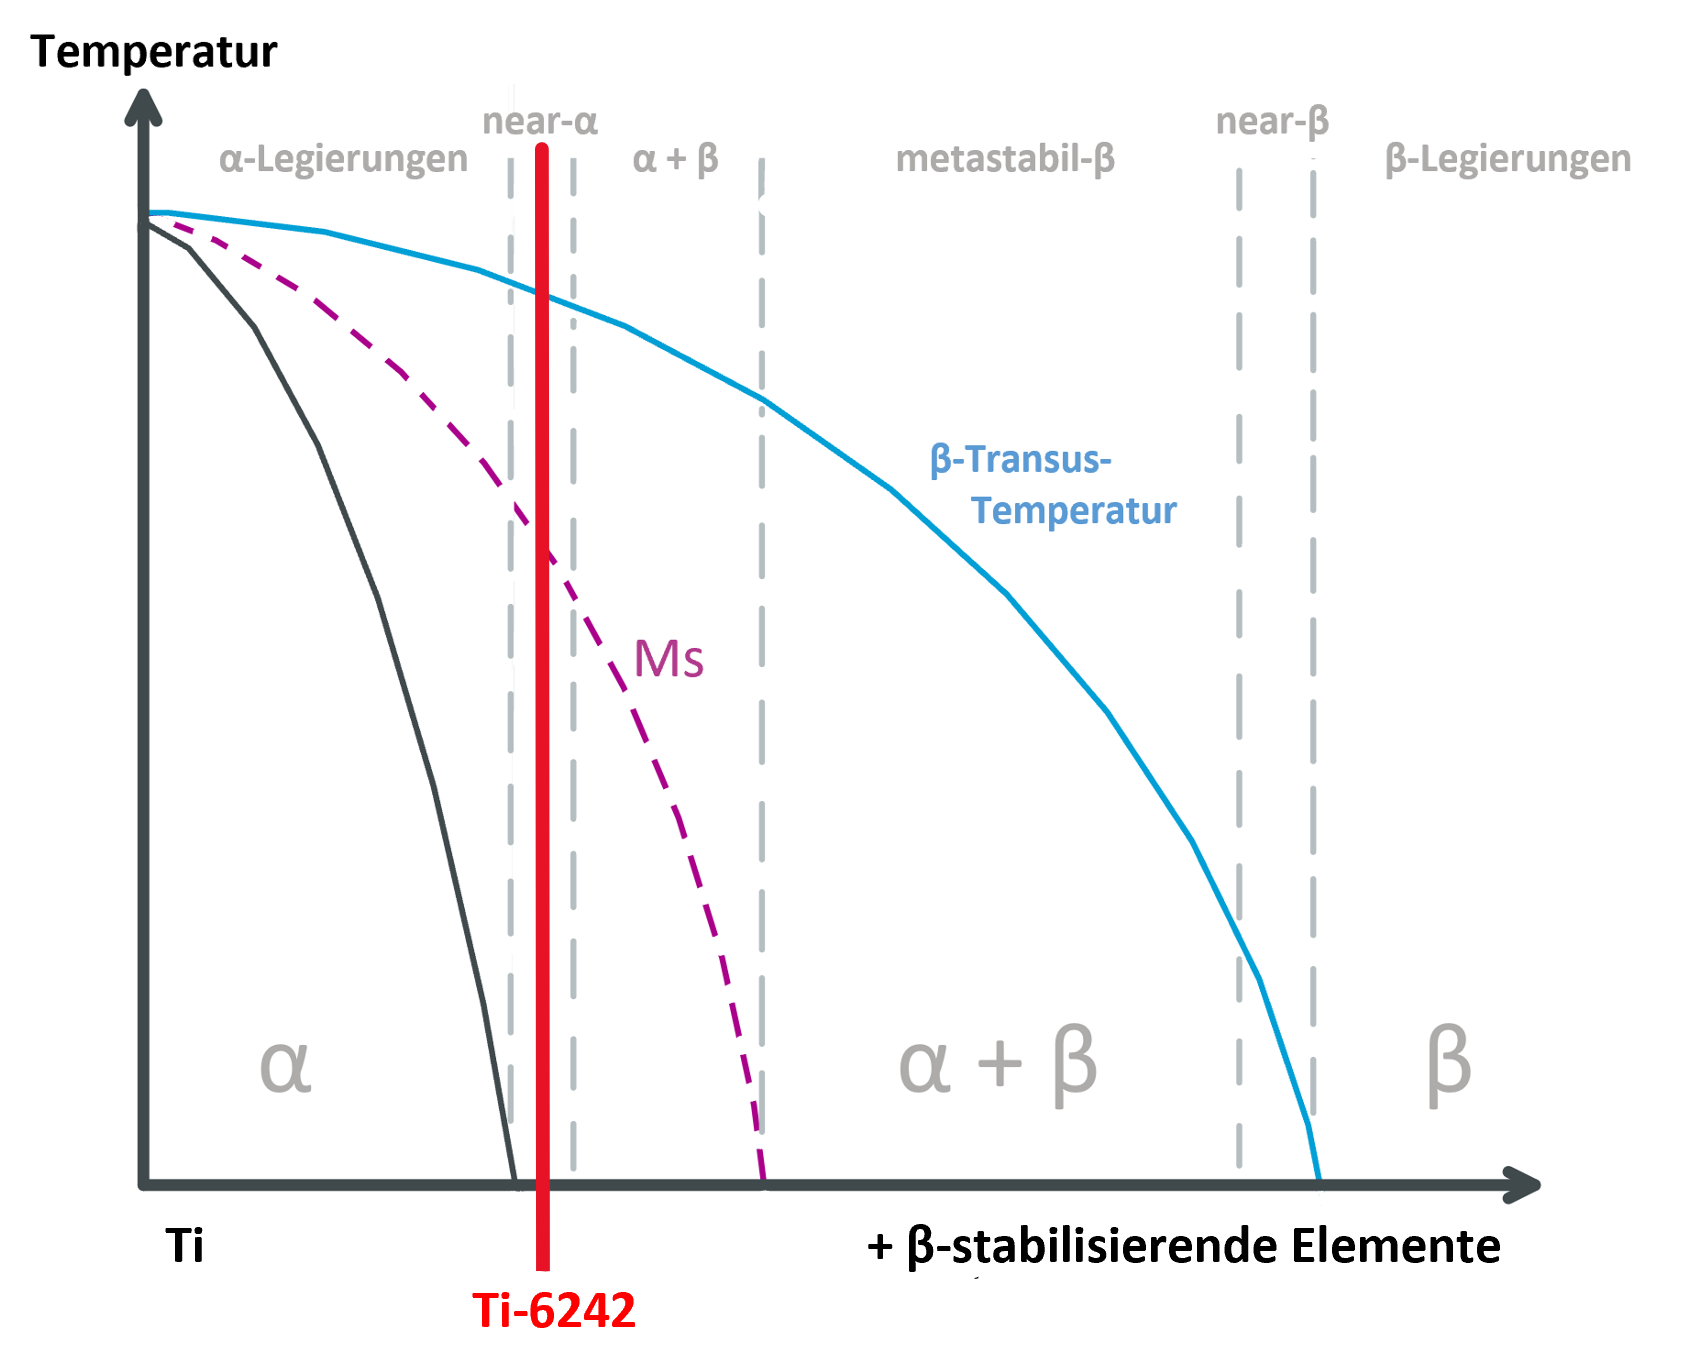
\includegraphics[width=0.5\textwidth]{Bilder/Phasendiagram}
	\caption{Phasendiagramm [Titanium Technical guide]}
	\label{PD-Ti6242}
\end{figure}





\begin{table}[H]
	
	\centering	
	\begin{tabular}{|l |c |c|}
		\hline
		\centering
		\hspace{20ex}Elements \hspace{20ex} & Min \%Gwt. & Max \%Gwt.\\
		\hline
		Aluminium&5,5&6,5\\
		Tin&1.80&2.20\\
		Zirconium&3.60&4.40\\
		Molybdenum&1.80&2.20\\
		Silicon &0.06&0.13\\
		Iron&-&0.25\\
		Oxygen&-&0.15\\
		Carbon&	-&	0.05\\
		Nitrogen&-&0.03\\
		Hydrogen&-&0.0125\\
		
		Titanium &&Remainder\\
		\hline
	\end{tabular}
	\caption{Zusammensetzung von Ti-6242 [Titanium : Technical guide]}
\end{table}


Die Ti6242S ist eine Optimierung von Ti6242, die erst in den 1970er Jahren  entwickelt wurde. Dieser wurde zusätzlich Silizium in kleinen Mengen zulegiert, um die Resistenz gegen Kriechen vor allem bei hohen Temperaturen durch die Bildung von Siliziden ($Ti_5Si_3$) zu erhöhen.  [Titanium and Titanium Alloys : Fundamentals and apps]. 

Verzeichnis : [Immanuel Freiherr von Thungen] - Immanuel Freiherr von Thungen. Effet dwell: relation microstructure-microtexture-propriétés mécaniquesdel’alliagedetitaneTi6242. Autre. ISAE-ENSMAEcoleNationaleSupérieuredeMécanique et d’Aérotechique - Poitiers, 2016. Français. NNT: 2016ESMA0027 .  tel-01486574
[Titanium and Titanium Alloys : Fundamentals and apps] Williams J. C., Belov A. F., eds.: Titanium and Titanium Alloys, Plenum Press, New York, USA, (1982) 


\subsection{Kristallstruktur}

Ti6242 wird klassischerweise in der bimodalen oder Duplex-Struktur eingesetzt die nach einer typischen Wärmebehandlung , erklärt in Abbildung \ref{WB} , erreicht  werden kann.

\begin{figure}[H]
	
	\centering
	
	{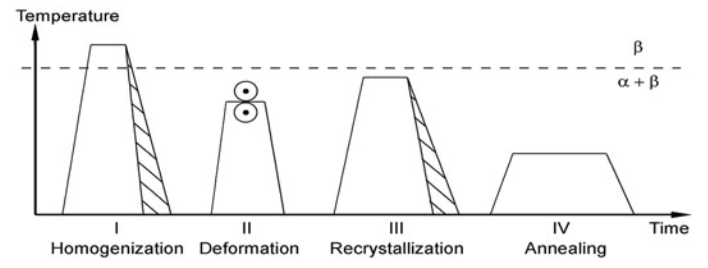
\includegraphics[width=1\textwidth]{Bilder/WB}}			
	\caption{Schematic processing route for bi-modal microstructures $\alpha$+$\beta$-titanium alloys )}
	\label{WB}
\end{figure}
Nach dem Deformationsvorgang wandelt sich bei der Erwärmung von Raumtemperatur  auf \hspace{1ex} T1<$T_{\beta}$  ein Anteil von der $\alpha$-Phase in $\beta$ um. Nach 1-2h werden die Werkstücke wieder auf Raumtemperatur luftgekühlt.
Dabei wandelt sich das $\beta$ unter Einfluss der Diffusion in $\beta$ + $\alpha$-Lamellen um.

\begin{figure}[H]
	\centering
	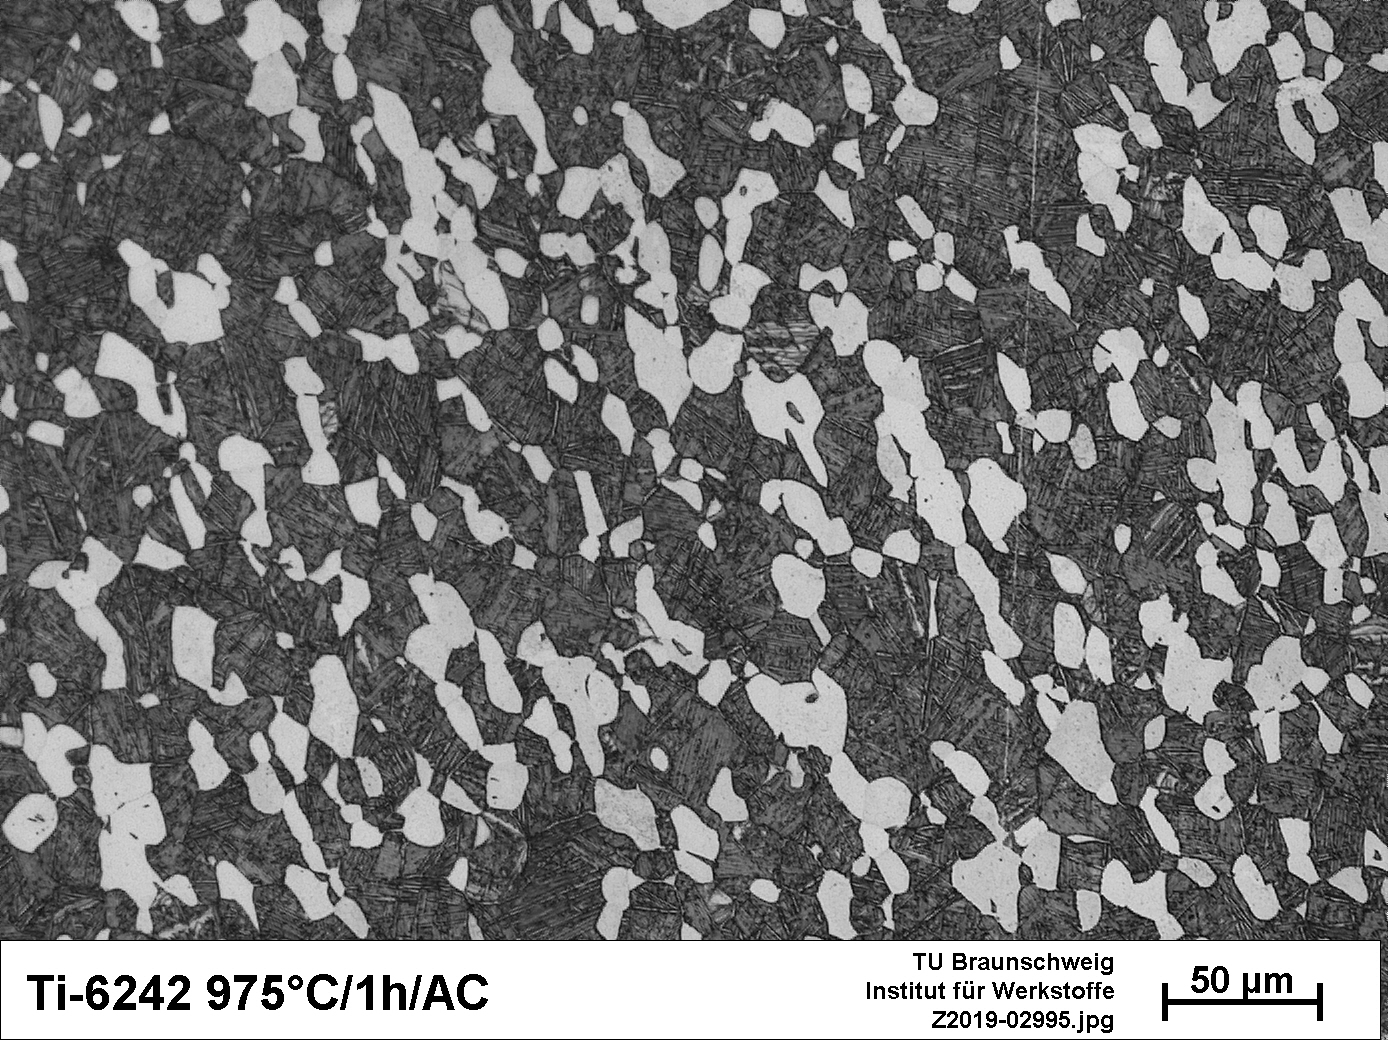
\includegraphics[width=0.9\textwidth]{Bilder/LM-975-1h-AC}
	\caption{}
	\label{L.M}
\end{figure}


Als letzte Wärmebehandlung wird klassischerweise  Ti6242 oder Ti6242S für  8 h bei 595$^\circ$C angelassen. Dieser Schritt sorgt dafür, dass sich $\alpha_2$ ($Ti_3Al$) in der $\alpha$-Phase ausscheidet und die dadurch weiter verstärkt. Der Temperaturbereich hängt dabei von der Solvus-Temperatur von $\alpha_2$ in $\alpha$, die ca. 650$^\circ$C beträgt.(Titanium lütjering )
Für besonders gute Kriechverhalten bei hohen Temperaturen, wird auch die Solvus-Temperatur von Si berücksichtigt, die knapp unter 600$^\circ$C liegt. Silizide ($Ti_5Si_3$) können sich aufgrund ihrer komplexen Kristallstruktur dann in den Korngrenzen ausscheiden und Kornbewegungen verhindern.


\begin{figure}[H]
	\centering
	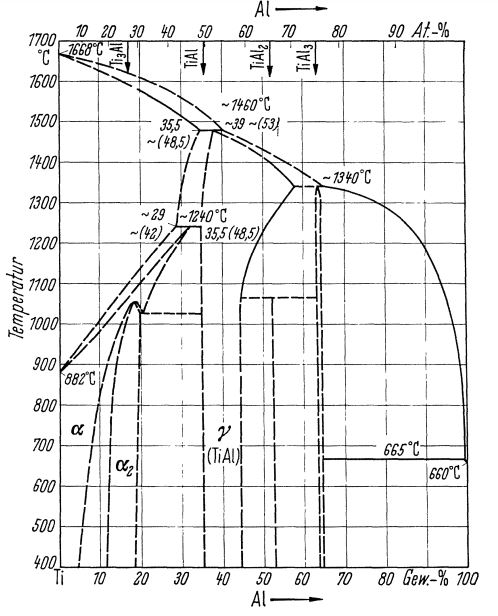
\includegraphics[width=0.6\textwidth]{Bilder/TiAl}
	\caption{Phasendiagramm von Ti-Al . [Titan Titanöegierungen, Ulrich Zwicker]}
\end{figure}
+ Phasendiagram Mo-Ti
Wärmebehandlungen von Ti6242 und deren Einflüssen werden in den nächsten Kapiteln noch genauer diskutiert.


\subsection{Physikalische und mechanische Eigenschaften }

Die Tabelle in Abbildung \ref{Phy.eig.} fasst ein paar physikalische Kennwerte vom Ti-6242 zusammen.
\newline
\textit{	Referenzen : 
	Metals Handbook, Vol.2 - Properties and Selection: Nonferrous Alloys and Special-Purpose Materials, ASM International 10th Ed. 1990.				
	Metals Handbook, Vol. 3, Properties and Selection: Stainless Steels, Tool Materials and Special-Purpose Metals, Ninth Edition, ASM Handbook Committee., American Society for Metals, Materials Park, OH, 1980.				
	Structural Alloys Handbook, 1996 edition, John M. (Tim) Holt, Technical Ed; C. Y. Ho, Ed., CINDAS/Purdue University, West Lafayette, IN, 1996. }

\begin{table}[H]
	\centering	
	\begin{tabular}{l c}
		
		Physikalische Eigenschaften & \\
		\hline
		Dichte& 4,54 g/$cm^3$\\
		Wärmeleitfähigkeit & 7 $W/mK$ \\
		Spezifische Wärmekapazität & 0.460 $J/gK$\\
		Schmelzpunkt & 1700^\circ C \\
		$T_{\beta}$ &  995^\circ C $\pm$ 15^\circ C \\
		\hline
		
	\end{tabular}
	\caption{Physikalische Kennwerte von Ti6242 : ???]}
	\label{Phy.eig.}
\end{table}


Die mechanischen Eigenschaften von Titanlegierungen, wie bereits im ersten Kapitel erklärt wurde, hängen auch stark von den verschiedenen Wärmebehandlungen ab, die die Gefügestruktur des Werkstoffes  verändern und so auch sein thermomechanisches Verhalten.
Als eine Near-$\alpha$Titan Legierung, ist Ti6242 zum größten Teil $\alpha$(90-95\%)(Siehe Phasendiagramm in Abbildung \ref{PD-Ti6242}). Da die Diffusionsrate bei $\beta$-Strukturen höher ist als bei $\alpha$Strukturen weist Ti6242 eine bessere Stabilität bei höheren Temperaturen auf. (Aerospace Materials and Material Technologies ) 

\begin{table}[H]
	\centering	
	\begin{tabular}{|c| c| c| c| c| c|}										
		\hline
		$T_{\beta}$ & Härte[HV] & E-Modul [Gpa]& YS [Mpa]&TS[Mpa]& El \% \\
		\hline
		995&340&114&990&1010&13\\
		\hline
	\end{tabular}
	\caption{Physikalische Kennwerte von Ti6242S [Titanium and Titanium alloys  : Fundamentals and apps.]}
	\label{Mec.}
\end{table}

Die $\alpha$-$\beta$-Transformationstemperatur $T_{\beta}$ von Ti-6242 liegt bei 995$^\circ$C $\pm$ 15$^\circ$C . Die Abweichung hängt  von den Anteilen der verschiedenen Legierungselementen ab. Wie bereits im ersten Kapitel beschrieben wurde, stabilisieren  Al, O , N und C die $\alpha$Phase und erhöhen im Gegensatz zu Mo  {$T_{\beta}$}.
Aufgrund des niedrigen Mo-Gehalts von Ti6242 liegt ihre Betat-trans-Temperatur oberhalb der von Reinem Titan, die bei 882 $\pm$ 2$^\circ$C liegt.


\begin{figure}[H]
	\centering
	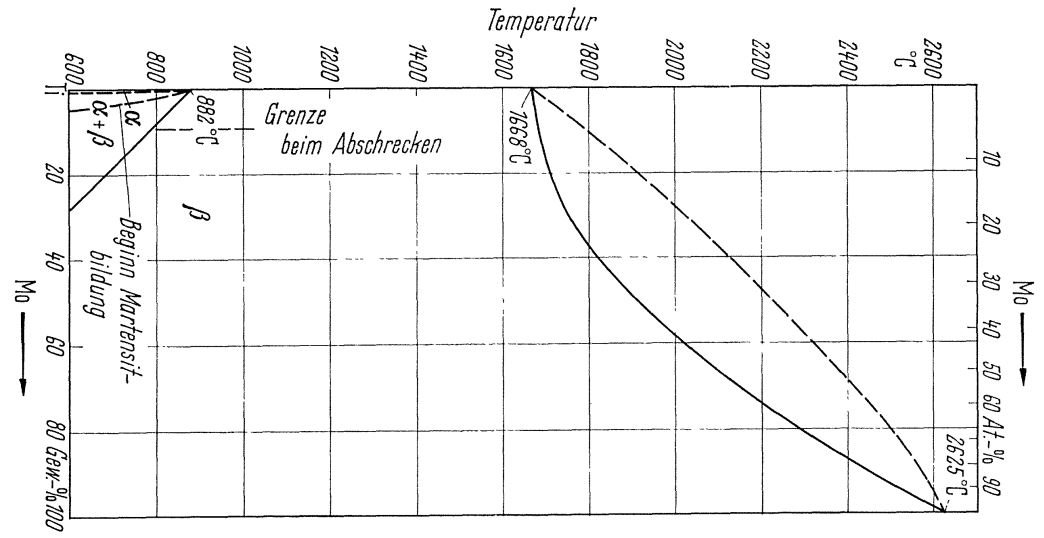
\includegraphics[width= 0.6\textwidth]{Bilder/TiMo}
	\caption{Phasendiagramm Ti-Mo [Titan titanlegierungen Zwickers]}
	\label{TiMo}
\end{figure}

\begin{table}[H]
	\small
	\tabcolsep=0.09cm
	\centering	
	\begin{tabular}{|c |c |c|c |c|}
		\hline
		\centering
		Thickness[mm] & Tensile strength [MPa] & Yield strengh [MPa] & Elongation[\%]& Reduction in Area [\%]. \\
		\hline
		25-50&1000&930&14&33\\
		102&1000&930&12&30\\
		205&1035&940&12&28\\
		330&1000&825&11&21\\
		
		\hline
	\end{tabular}
	\caption{Elatische Eigenschaften bei Raumtemperatur von Ti6242Si (Annealed 1h 954$^\circ$C/AC + 8h/600$^\circ$C/AC )  [Titanium : Technical guide]}
	\label{Mecprop}
\end{table}






\%	Für den Einsatz in der Luftfahrt sind aber auch spezielle mechanische  Eigenschaften wie zB eine hohe Festigkeit und Duktilität, eine hohe Kriech- und Korrosionsbeständigkeit bei relativ hohe Temperaturen gesucht.   

Alle sekundären Fertigungsverfahren, die für die Herstellung von Bauteilen erforderlich sind   wie zB. Biegen, Fräsen und Schweißen können Eigenschaften von Titan oder Titanlegierungen stark beeinflussen  und müssen daher mitberücksichtigt werden.




\subsection{Verwendung}


Die Kombination von der Festigkeit der ($\alpha$+$\beta$)-Gefüge mit der relativ hohen Kriechbeständigkeit der $\alpha$-Strukturen macht von Ti6242/Ti6242S eine \textit{High Temperature Ti-Alloy}.

Wegen dieser Eigenschaften werden Ti6242/Ti6242S hauptsächlich in der Luftfahrt eingesetzt. Vor allem bei rotierenden Teilen im Triebwerk, wo  hohe Kriechbeständigkeit, Ermüdungsresistenz  neben eine hohe metallurgische Stabilität bei hohen Temperaturen erforderlich sind. 
Ti6242-Bauteile können in Temperaturen bis zu 500-550$^\circ$C eingesetzt werden. [Titanium and itanium alloys : fundamentals and apps]
Ti6242 wird z.B. in der Herstellung von Hochdruckverdichterschaufeln, Turbinenschaufeln und Nachbrennern verwendet, wo neben den oben erwähnten Eigenschaften auch die Korrosionsbeständigkeit bei hohen Temperaturen erforderlich ist. \newline



\begin{figure}[H]
	\centering
	\subfloat[Compressor spoolfor GE CF6 class engine using inertia welding toconnect the individual stages:front (smaller)five stages: Ti–6Al–4V; rear two stages:Ti-6242 ]
	{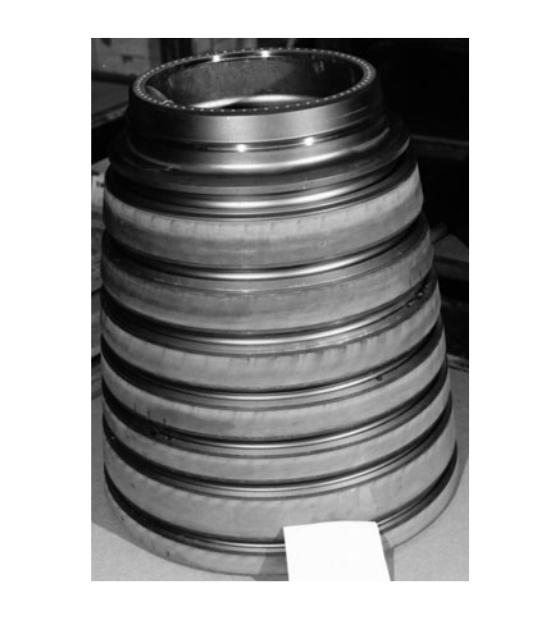
\includegraphics[width=0.45\textwidth]{Bilder/Compressor spool}}
	\hspace{1ex}
	\subfloat[Impeller used in asmall engine for regional jets, diameter 35 cm. The alloy is Ti-6242 with a bi-modalmicrostructure]
	{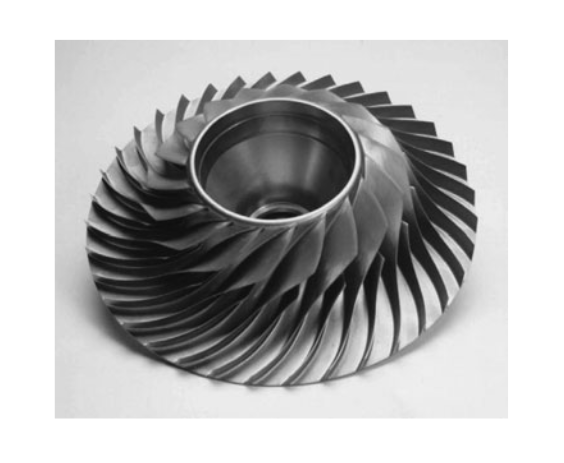
\includegraphics[width=0.45\textwidth]{Bilder/Impeller}}
	
\subfloat[Bläser und Verdichter des JT9D-Triebwerkes. das zu 28 \% des Fluggewichtes aus
	Titan und Titanlegierungen besteht. Bläser aus TiAI6V4. Verdichter mit zunehmender
	Temperatur aus TiAI6V4, TiAl811folVI und TiAl6Zr4Sn2Mo2 [T 19b].]
	{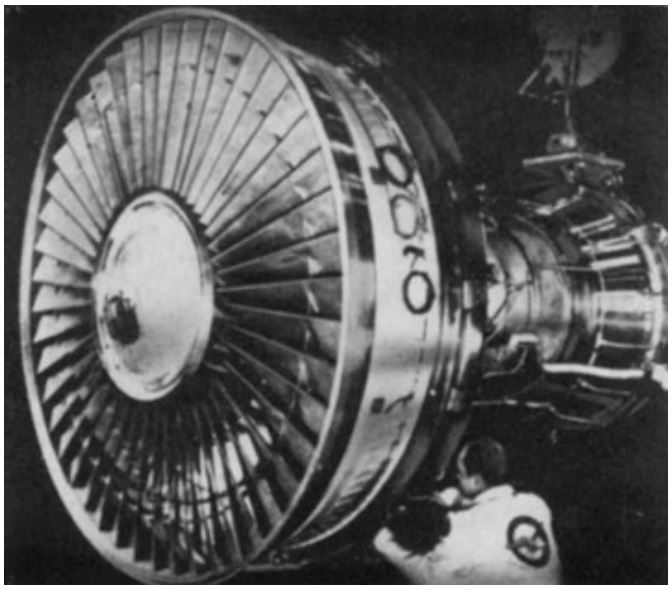
\includegraphics[width=0.45\textwidth]{Bilder/Titan}}
	\caption{Beispiele von Einsatzbereiche von Ti-6242 (Aerospace Materials and Material Technologies )}
\end{figure}




